\documentclass[11pt,a4paper]{article}

\usepackage[utf8]{inputenc}
\usepackage[T1]{fontenc}
\usepackage{lmodern}
\usepackage[margin=2.5cm]{geometry}
\usepackage{graphicx}
\usepackage{booktabs}
\usepackage{tabularx}
\usepackage{array}
\usepackage[font=small]{caption}
\usepackage{url}
\usepackage[hidelinks]{hyperref}

\renewcommand{\arraystretch}{1.15}
\newcolumntype{L}{>{\raggedright\arraybackslash}X}
\setlength{\parskip}{0.5em}
\setlength{\parindent}{0pt}
\graphicspath{{figures/}}
\renewcommand{\topfraction}{0.9}
\renewcommand{\bottomfraction}{0.8}
\renewcommand{\textfraction}{0.1}
\renewcommand{\floatpagefraction}{0.8}
\setcounter{totalnumber}{4}

\begin{document}

\begin{center}
{\Large Two thesis directions for data-quality controls}\\[0.4em]
{\large Proposal overview and pilot results}\\[0.8em]
Tomash Oosterbaan\\
MSc Artificial Intelligence, University of Groningen\\
Graduation project context: Avanade and Rabobank\\
October 2026
\end{center}

\section{Motivation and scope}

Data from a new source is rarely ready for immediate use. Before a bank uses a new file in reports, models or decisions, a data team checks it. Required fields must be present, values must have the right type, codes must come from an agreed list and known business rules must hold. Long Tran described this kind of work in his context at Rabobank: technical validation, business rules, monitoring thresholds, pass and fail checks, and manual investigation of exceptions \cite{tran}. A public Rabobank case study also mentions missing data and differences between information providers as practical problems \cite{alderse}. These observations motivate the examples in this document. They are not a description of Rabobank systems, and no Rabobank data is used. All data in this work is public.

The question behind both directions is the same: can AI help such a team find data problems that its existing checks miss, and how would the team know whether to trust it? AI can play two different roles here. It can act as a detector, a model that looks at the data and points at values that seem wrong. Or it can act as a writer of validation rules: it proposes rules that a person can read, approve and then run like any other check. Direction A studies the first role. Direction B studies the second.

Both directions were explored with a pilot study. The first pilot compared error detectors on public tables. Its results led to the second pilot, which tests AI-written rules on public financial filings against a set of rules written by experts. This document explains both directions, what we did, which datasets we used and why, what the results show, and what they do not show. The pilots were exploratory. They used small samples and limited computing power, so the numbers are indications and not conclusions.

\section{Terms used in this document}

Table~\ref{tab:terms} explains the terms that return in both directions.

\begin{table}[htbp]
\centering
\small
\begin{tabularx}{\textwidth}{@{}p{3.1cm}LL@{}}
\toprule
Term & Meaning & Example \\
\midrule
Validation rule & A fixed check that a value or record must pass. & ``The repayment status must be one of the codes $-2$ to $9$.'' \\
Detector & A method that marks values as suspicious, often learned from data. & A model predicts a monthly bill from the other fields and flags bills far from the prediction. \\
Alert & One item that a control marks and that a person may have to look at. & ``Customer 1043, field BILL\_AMT1, value 24{,}000.'' \\
Injected error & An error we put into the data on purpose, so we know exactly where it is. & A bill of 2{,}400 is changed into 24{,}000. \\
Reference (ground truth) & What we use to decide whether an alert is correct. & The list of injected errors, or the messages of an official rule. \\
Review capacity & How many alerts a person can investigate per batch. & 20 alerts per delivery of 800 records. \\
False alarm & An alert on a value that is in fact correct. & A legitimate negative amount flagged by a ``never negative'' rule. \\
\bottomrule
\end{tabularx}
\caption{Terms used in both directions.}
\label{tab:terms}
\end{table}

\section{Direction A: the added value of data-quality detectors}

\subsection{Core idea and practical setting}

Consider a team that onboards a monthly file with customer credit data. Its rules already reject missing fields, numbers that cannot be read and codes that are not on the agreed list. Some errors pass these rules. A monthly bill can be copied from the wrong month and still be a valid number. An education code can be replaced by another valid code. The team considers adding a statistical or AI-based detector to find such cases. Before it does, it wants to know two things: does the detector find errors that the rules miss, and how many extra alerts does it create?

This is an old question in data cleaning. Abedjan et al.\ ran several detection tools on real datasets with known errors and found that no single tool came close to finding all of them. Combining tools found more, but every tool also added alerts that a person had to check \cite{abedjan}. Libraries such as Deequ make rule-based checks easy to define and run \cite{deequ}, and newer detectors learn patterns or relationships from the data itself \cite{cdc,lucario,riolu,autotest}. What the team needs is evidence of the extra value of such a detector in its own situation, compared with the checks it already has.

My earlier proposal focused on a related question: whether the best detector changes when errors occur in different ways. Jung et al.\ separate the type of an error (what happens to a value) from its mechanism (which values are affected) \cite{taberr}. Errors can be placed completely at random (ECAR), depending on another field such as the source system (EAR), or depending on the original value itself, for example more errors in large amounts (ENAR). The CURED demonstrator combines this error model with the CDC detector \cite{cured,cdc}. The pilot showed that a more basic question had to be answered first: whether an extra detector adds anything at all once reasonable checks are in place. The direction was therefore widened to the added value of detectors under limited review capacity.

\subsection{What we did}

The first pilot used public data only. Three complete tables from the UCI repository were used for controlled experiments (Table~\ref{tab:a-data}). Each table contributed 800 evaluation records, and separate historical records were used to learn normal values and relationships. The outcome columns of these tables (default, campaign response and wine quality) were never given to the detectors and are not data-error labels.

\begin{table}[htbp]
\centering
\small
\begin{tabularx}{\textwidth}{@{}p{3.6cm}p{2.2cm}L@{}}
\toprule
Dataset & Size & Why it was used \\
\midrule
Default of Credit Card Clients \cite{uci-credit} & 30{,}000 rows, 25 fields & Credit limits, monthly bills, payments and repayment codes. Closest to a bank credit file. \\
Bank Marketing \cite{uci-bank} & 41{,}188 rows, 21 fields & Customer and contact data with many categorical fields, so valid but wrong categories can be tested. \\
Wine Quality, white \cite{uci-wine} & 4{,}898 rows, 12 fields & Mainly numerical and not financial, to see whether the behaviour repeats outside finance. \\
Published benchmarks \cite{autotest,raha} & various & Auto-Test RT and ST values labelled by the publishers, date, IP and code fields, Hospital and Beers. These provide labels that we did not create ourselves. \\
\bottomrule
\end{tabularx}
\caption{Data used in the first pilot.}
\label{tab:a-data}
\end{table}

We changed selected values in a copy of each table and recorded exactly which cells were changed. A first round of 630 scenarios covered missing fields, invalid types, invalid codes, scale changes and plausible replacements. A second round of 360 scenarios focused on changes that pass the basic rules, such as a bill copied from the wrong month or a category replaced by another valid category. These were run with two amounts of context (four target fields only, or all permitted fields), giving 720 combinations. Another 135 scenarios changed characters in dates, IP addresses and codes. Each change was applied to 1\%, 5\% or 10\% of eligible values, under ECAR, EAR and ENAR, with five random seeds.

The methods ranged from simple to recent research systems. The existing controls were explicit rules, statistical checks learned from history (unusual ranges and rare categories), and simple prediction models (Ridge regression for numbers, logistic regression for categories). On top of these we added CDC, which predicts a value from the other columns and flags values outside a calibrated range \cite{cdc}; dBoost, a statistical outlier method; LUCARIO and RIOLU, which learn common formats and ranges without labels \cite{lucario,riolu}; Auto-Test, which applies constraints learned in advance from a large collection of tables \cite{autotest}; Raha, which learns from a few labelled examples \cite{raha}; a tree-based prediction model; and a small local experiment inspired by ZeroED, in which a language model helps label values \cite{zeroed}.

The evaluation followed the order in which a team would work. First all existing controls were run. Then a detector was added, and we counted three things: how many changed values it found that the existing controls did not, how many extra alerts it created, and how many extra changed values a reviewer would actually see if only 20 alerts per 800 records can be checked. The last number is the net benefit. It can be negative, because the extra alerts can push correct findings of the existing controls out of the limited review list. Engineers in practice describe exactly this problem as alert fatigue \cite{shankar}.

\subsection{Results}

The rules already found every injected missing value, invalid type and invalid code in the 360 relevant scenarios of the first round. More advanced detectors are therefore only interesting for errors that pass the rules.

For those errors, detectors did find extra changed values, but at a high price. Figure~\ref{fig:a} shows three typical cases at a 5\% error rate. CDC found between 11 and 21 of the 40 changed values that the rules, statistics and Ridge model missed, but it also created between 520 and 900 extra alerts. With 20 reviews per batch, the net benefit was $+0.4$ changed values for Bank, $0$ for Credit and $-1.0$ for Wine. When we added a simple logistic regression for categories to the existing controls, the small gain for Bank disappeared ($-0.4$ or $0$ depending on the threshold), and Credit became $-0.2$. Part of what looked like the value of an advanced detector could be achieved by a cheap model.

\begin{figure}[htbp]
\centering
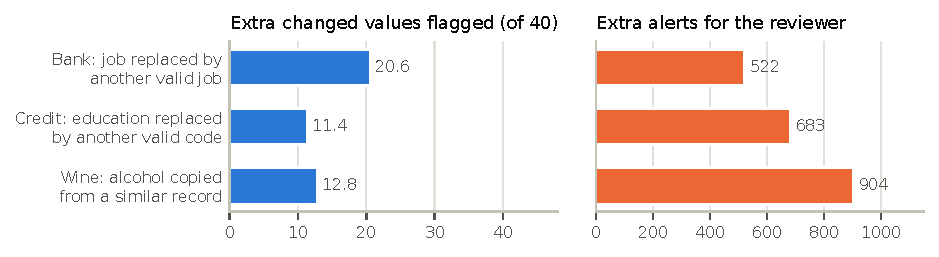
\includegraphics[width=\textwidth]{fig_a_increment.pdf}
\caption{First pilot, CDC added to rules, statistics and a Ridge model. Error rate 5\%, random placement, all permitted fields, mean of five runs. Left: changed values found that the existing controls missed. Right: extra alerts. The changes were made by us; they are not verified real errors.}
\label{fig:a}
\end{figure}

On the published benchmarks the picture was similar. In the RT and ST collections the publishers mark 41 and 45 values as errors. Auto-Test on its own flagged 35 RT and 23 ST values, of which 10 and 6 matched these labels. With 25 review slots, adding Auto-Test to generic statistical checks gave 5 extra correct findings on RT and 4 on ST. Against a stronger pattern-based check the gain shrank to 3 and 1, and if the existing alerts were reviewed first, the gain was 0. RIOLU found all 40 changed dates in one setting, but a standard date check would catch most of these too, and RIOLU needs at least 385 values per column, so it could only run on 74 RT and 46 ST columns. Finally, where the original source file was still available, a simple comparison of source and copy found every change. A learning method cannot improve on that.

\subsection{What we can do with these results}

The first pilot shows that the value of a detector depends less on the detector itself than on the situation: how strong the existing checks are, which errors occur, what information the detector may use, and how many alerts a person can handle. A thesis in this direction would ask:

\begin{quote}
Under which error conditions do automatically inferred and contextual data-quality detectors provide useful additional detections beyond conventional and simple predictive controls when review capacity is limited?
\end{quote}

The planned engineering artefact was a Data Quality Evaluation Service: a team registers a new table and its known rules, the service tests candidate detectors with controlled errors and reports extra findings and extra alerts under a given review capacity. The first version already runs end to end.

The direction also has weaknesses. Comparing detectors and the human cost of checking their output was already studied by Abedjan et al.\ \cite{abedjan} and in benchmarks such as REIN \cite{rein}, so the novelty would lie in a careful conditional comparison, not in a new idea. All errors were made by us, so the results are about detecting changes, not about real mistakes. Three tables are three sources, which limits general claims. And the role of AI is small: most tested methods are statistical, and the language-model part was a small local experiment. These points led to the second direction, in which the AI part is central and the reference is written by independent experts.

\section{Direction B: can AI-written validation rules be trusted?}

\subsection{Core idea and practical setting}

Suppose a credit team wants to use the financial statements that business clients publish. A new feed arrives with thousands of figures per company. The team has some checks, for example that every figure has a period and a currency. An analyst asks an AI model to suggest more checks, and within a minute it returns twenty rules, such as ``total assets must equal liabilities plus equity'' or ``a figure reported twice for the same period must have the same value''. Some of these rules are useful. Others are wrong in ways that are hard to see. A rule can look reasonable and still flag hundreds of correct figures per company. And if the analyst asks again tomorrow, the model may write a different rule.

Writing rules with language models is not new. LeDQeR generates rules from erroneous records and filters out rules that misfire on clean data \cite{ledqer}. Akella et al.\ let a model write Python validators with retrieval and guardrails \cite{akella}. AuDQ lets agents discover rules for banking and retail data, which human reviewers then rate \cite{audq}. These studies judge generated rules against labelled cells or human ratings. The AuDQ authors note that neither of their datasets ``ships with a reference rule set to compare against'' \cite{audq}. Stress-testing checks by injecting errors is not new either: Homayouni et al.\ used it to test ETL checks in data warehouses, and JENGA used it to improve the schema of a machine-learning pipeline \cite{homayouni,jenga}.

Closest to our idea, Alexander et al.\ compared validation tests written by GPT-3.5 and GPT-4 with a gold-standard suite written by an experienced data scientist, and ran every setting five times to measure consistency \cite{alexander}. Their reference is one suite for one dataset, written for the study. What we did not find is a test of AI-written rules against a large public rule set that a committee of experts wrote and approved independently of any study, with official test cases on real financial data, where both the expert rules and the AI rules are executed on the same filings. Such a rule set gives three things: a reference for what a good rule should find, a strong existing control to compare against, and a realistic picture of a team that already has rules. The idea of direction B is to use exactly that, and to add a governance step: no AI rule is used until it has passed a stress test, an alert limit and a human decision. This step is needed because automatically found rules are often wrong. Martin et al.\ found that the share of false constraints produced by discovery algorithms is ``rarely below 95\%'' \cite{martin}, and people tend to accept automated suggestions too easily \cite{parasuraman}.

\subsection{Data: SEC filings and the DQC rules}

American listed companies file their financial statements with the SEC in XBRL, a machine-readable format. Every number in a filing is a fact with a label from a shared dictionary (the taxonomy), a period, a unit and a precision. For example: \texttt{Revenues} $=$ 5{,}000{,}000, from 1 January to 31 December 2024, in US dollars, rounded to thousands. This makes each number checkable by rules.

The XBRL US Data Quality Committee (DQC) publishes about 200 approved rules for these filings, free of charge \cite{dqc}. Examples are rules that flag a negative value for an element that cannot be negative, or a subtotal that does not match its parts. Each rule has a written description, an implementation, and official test cases on real filings with the messages the rule is expected to give. The rules run in the open-source XBRL processor Arelle \cite{arelle}. Accounting research has shown that XBRL filings contain real errors, for example signs entered the wrong way because of confusion about debit and credit \cite{debreceny}.

We used three public sources (Table~\ref{tab:b-data}). This domain was chosen because it is financial, public and real, and because it has what most studies on AI-written rules lack: an expert rule set with official tests. It also contains corrections. When a company finds a mistake, it can file an amended report, and comparing the original and the amendment shows which numbers changed. Brown et al.\ used such amendments as signals of misreporting at company level \cite{brown}.

\begin{table}[htbp]
\centering
\small
\begin{tabularx}{\textwidth}{@{}p{3.6cm}p{3.6cm}L@{}}
\toprule
Source & What we used & Role \\
\midrule
SEC Financial Statement Data Sets \cite{fsds} & 10 quarters (2023 to mid-2025): 68{,}875 filings, 1{,}294 pairs of original and amended report & Real correction candidates, and patterns to make injected errors realistic \\
EDGAR XBRL filings & 240 filings: 120 never corrected, 120 later corrected & The data every control and AI rule is run on \\
DQC rules and test suite \cite{dqc} & 185 US rules, 472 official test cases, rulesets 2023 to 2025 & What the expert rules report; official rules as an existing control \\
\bottomrule
\end{tabularx}
\caption{Data used in the second pilot.}
\label{tab:b-data}
\end{table}

\subsection{What we did}

We kept five questions apart, because each needs a different reference (Table~\ref{tab:e}). Mixing them would make the results hard to interpret: a rule can reproduce an expert rule well and still add nothing, or catch many errors and still be unusable because of its alerts.

\begin{table}[htbp]
\centering
\small
\begin{tabularx}{\textwidth}{@{}p{0.7cm}LL@{}}
\toprule
 & Question & Reference \\
\midrule
E1 & Can the AI reproduce an official expert rule from its written description? & Messages of the official rule on the official test filings \\
E2 & Which injected errors does each control catch? & The errors we injected \\
E3 & Does a control flag numbers that were later corrected? & Corrections from amendments (candidates, not proven errors) \\
E4 & What does AI add beyond the existing controls? & Injected errors missed by DQC, statistics and generic checks \\
E5 & Is the result stable, and how many alerts does it cost? & Repeated generations; alerts on filings that were never corrected \\
\bottomrule
\end{tabularx}
\caption{The five evaluation questions of the second pilot.}
\label{tab:e}
\end{table}

Real corrections (E3). We first looked at what the amendments actually correct. Of the 1{,}294 pairs, 631 changed at least one number. Most of these were accounting restatements, not typing errors. In a document-based check of 20 targeted corrections, six were confirmed as accounting or classification corrections and none as a typing, sign or scale error. This check was assisted by an AI model and has not yet been verified by a person. We therefore treat corrections as candidates, not as proven errors.

Injected errors (E2 and E4). We then injected seven kinds of errors (Table~\ref{tab:ops}). Their placement and size were based on the corrections, for example which elements are often corrected and by what ratio values change. Each variant of a filing contains one injected error, so we know exactly what should be found. In the first run we changed only one copy of a number that appears several times in a filing. A simple duplicate check then caught almost everything, which said more about our injection than about the controls. In the final run all copies were changed. Injected errors are a standard way to test checks: in software testing, the detection of artificial faults is related to the detection of real faults \cite{just}. They do not replace real errors, which is why E3 is kept as a separate question.

\begin{table}[htbp]
\centering
\small
\begin{tabularx}{\textwidth}{@{}p{3.4cm}L@{}}
\toprule
Error & Example \\
\midrule
Sign flipped & Net income of 120 becomes $-120$. \\
Value x1000 & 4{,}500 (in thousands) is entered as 4{,}500{,}000. \\
Amount changed & A value changes by a ratio seen in real corrections. \\
One digit changed & 18{,}340 becomes 18{,}390. \\
Wrong element & An amount is reported under a related but wrong label, based on observed confusions. \\
Periods swapped & This year's value and last year's value are exchanged. \\
Fact removed & A reported number is missing. \\
\bottomrule
\end{tabularx}
\caption{The seven injected error types.}
\label{tab:ops}
\end{table}

Existing controls. Four kinds of controls were run on every filing: generic checks (for example duplicates with different values), statistical checks learned from 2023 and 2024 filings of other companies (unusual sign, unusual size, unusual jump between periods), a naive rule that amounts are never negative (to show what a careless rule costs), and the official DQC rules in Arelle.

AI as rule writer. Two open-source language models wrote rules as Python code: Qwen2.5-Coder-7B and Qwen3-8B \cite{qwen25coder,qwen3}. They ran locally on a normal processor, so no data was sent to an external service and no costs were made. They wrote rules in three ways. In translate mode, the model received the written description of a DQC rule and had to implement it (E1). In discover mode, it received a sample of a filing and had to propose useful rules. In gap-closing mode, it was told which kinds of injected errors the existing controls missed on development filings and had to write rules for them. Rules that crashed got one repair round. All generated code ran in a sandbox: a restricted, separate process without network access. Every prompt and answer was logged.

AI as judge. As a comparison, Qwen3-8B also read a table of facts from a filing and listed up to ten numbers it found suspicious. This is the detector role from direction A, and it is how most recent studies use language models on financial tables \cite{finauditing,secfintables}.

Fair testing. Filings were split into a development part and a test part. AI rules were only evaluated on test filings that no model had seen. For E1, rules were split by release date: rules published before the models could have appeared in their training data, rules published after both models could not. Before running anything, we fixed an approval policy: a rule set may only be considered if it gives at most one alert per never-corrected filing, catches at least 20\% of the injected errors that the existing controls miss, and gives the same result when run again.

\subsection{Results}

Reproducing expert rules (E1) and stability (E5). Figure~\ref{fig:e1} shows the results. For rules published before the models, both found about 41\% of the official messages. For rules published after the models, this dropped to 3\% for Qwen2.5-Coder and 13\% for Qwen3. Most rules scored 0\%, a few scored 97 to 100\%. A rule that we translated by hand found 15 of 16 messages, so the low scores are not caused by the test setup. The main failure types were code that assumed columns that do not exist, rules that ran but flagged nothing, output that was cut off, and descriptions that refer to lists the model never saw. Writing the same rule three times often gave very different results: for Qwen3, between 0\% and 100\% for two of the nine rules. One good AI rule therefore says little. A generated rule must be stored, versioned and tested like any other code.

\begin{figure}[htbp]
\centering
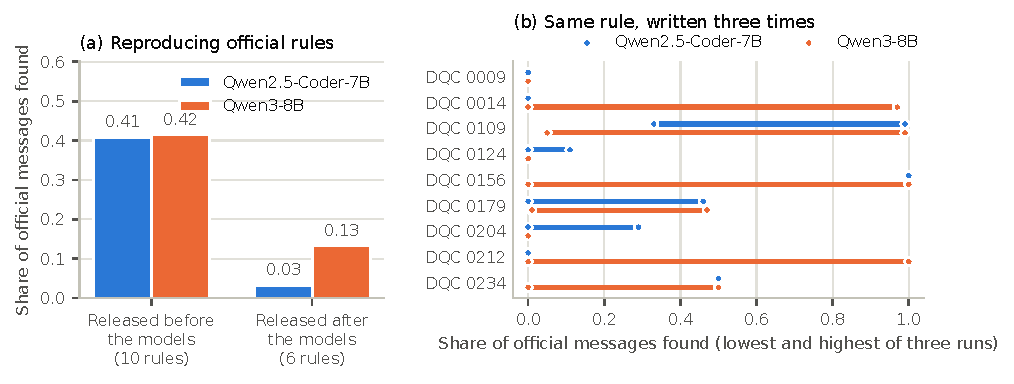
\includegraphics[width=\textwidth]{fig_b_e1_e5.pdf}
\caption{Second pilot. (a) Share of official DQC messages found by rules that the models wrote from the rule descriptions, split by whether the rule was published before or after the models. (b) Lowest and highest result of three generations of the same rule.}
\label{fig:e1}
\end{figure}

Injected errors (E2). Figure~\ref{fig:catch} shows which errors each control caught on 12 test filings where all controls, including the official DQC rules, could be run. The DQC rules caught 64\% of swapped periods and 50\% of x1000 errors, but only 17 to 25\% of the other types and none of the removed facts. The statistical period-jump check caught x1000 errors well and nothing else. The best AI rule set caught sign errors about as well as the naive ``never negative'' rule, and for the same reason.

\begin{figure}[htbp]
\centering
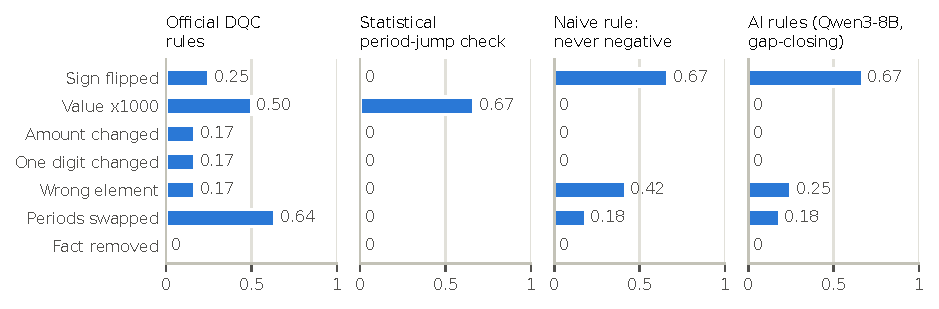
\includegraphics[width=\textwidth]{fig_b_catch.pdf}
\caption{Share of injected errors caught per error type, on the 12 test filings where official DQC could be run (83 variants).}
\label{fig:catch}
\end{figure}

Added value and alerts (E4 and E5). Together, the existing controls caught 27 of the 83 injected errors. The best AI rule set added 6, but gave on average 458 alerts on a filing that was never corrected. Figure~\ref{fig:alerts} puts these numbers side by side. The official DQC rules gave 1.8 alerts on such a filing. The AI rule sets that caught something produced between 36 and about 1{,}000 alerts per filing; most other AI sets crashed or caught nothing. Under the approval policy, none of the nine AI rule sets would be accepted. Of the five rule sets that failed in the sandbox, one round of automatic repair made one usable.

\begin{figure}[htbp]
\centering
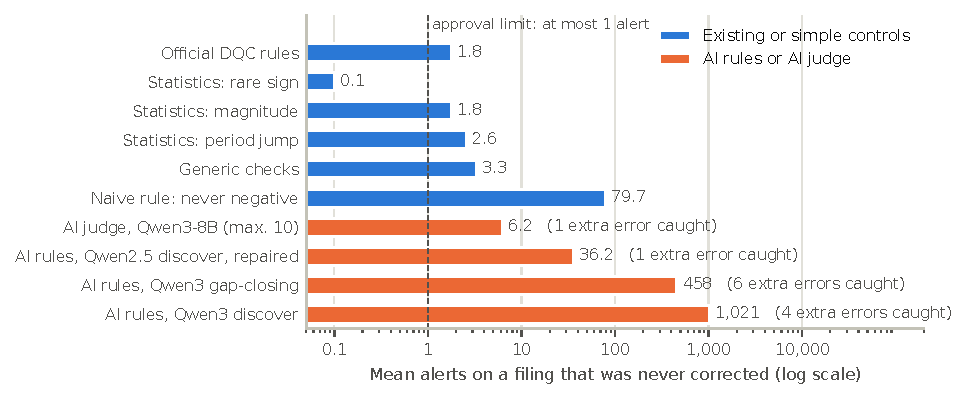
\includegraphics[width=\textwidth]{fig_b_alerts.pdf}
\caption{Mean alerts on test filings that were never corrected (66 filings; official DQC on 12; AI judge on 6 and limited to 10 flags). For AI sets, the number of injected errors caught beyond the existing controls is given in brackets (83 variants; AI judge 42). Log scale.}
\label{fig:alerts}
\end{figure}

The alerts show where the models went wrong. In the discover set of Qwen3, two rules caused most alerts. One compared the period type of each fact, stored as ``instant'' or ``duration'', with a list in which the SEC codes it as ``I'' or ``D'', so almost every fact was flagged. The other expected dimension names in a format our data does not use. In the gap-closing set, most alerts came from a rule that assumed that elements with a debit balance can never be negative. In XBRL that is not true: the balance type tells how an element adds up, not that its value must be positive \cite{debreceny}. These are domain mistakes, not programming mistakes, and a reviewer without XBRL knowledge would probably not see them.

AI as judge. The judge caught 2 of 42 injected errors and gave about six flags per never-corrected filing. Part of this is a limitation of the setup: to fit within the model's input limit, it saw at most 120 facts per filing, which included only 19 of the 42 injected errors. Even so, it caught 2 of these 19.

Real corrections (E3). On numbers that were later corrected, the official DQC rules flagged 1.6\% (129 located facts), and the statistical checks 0.1 to 0.6\%. One AI set flagged 92.6\% of the corrected numbers, but only because it flagged almost everything. A result on real corrections is meaningless without the number of alerts next to it.

\subsection{Engineering artefact}

The pilot produced a working command-line tool, \texttt{dqstress}, that follows the steps a team would take. The team registers a source, runs its existing controls, and stress-tests them with injected errors to see which error types slip through. It can then ask a local model to propose rules for those gaps. Each proposal is run in the sandbox, tested on held-out data and checked against the approval policy. A person records the decision, and the tool writes a report with the evidence: which errors the rule catches, how many alerts it gives on clean data, and whether repeated runs agree. For the credit team in the example, this turns ``the AI suggested twenty rules'' into a list of rules with evidence, of which perhaps none or a few are worth adopting. The tool does not change data, does not connect to production systems and does not approve anything by itself.

\subsection{What we can do with these results}

The pilot gives a clear but preliminary answer for small local models: they can sometimes reproduce an expert rule, they do so unstably, and the rules they invent add little beyond the expert rules at a high alert cost. This does not show that AI-written rules are useless. Larger open models may do much better, the prompts were not tuned (on purpose, to avoid tuning on the test data), and the rules were written in Python on a simplified table instead of in the DQC rule language on the full filing. What the pilot does show is that the evaluation design works and that it measures the things a team needs to know. The working research question is:

\begin{quote}
To what extent can LLM-generated validation rules provide reliable and reproducible error detection beyond expert-defined data quality controls in financial filings?
\end{quote}

My supervisors suggested three to five datasets. Table~\ref{tab:plan} shows a plan that keeps the same design in each case: public data, a public expert rule set, and injected errors. The European ESEF filings are closest to a Dutch bank, because they use IFRS like European companies do.

\begin{table}[htbp]
\centering
\small
\begin{tabularx}{\textwidth}{@{}p{3.3cm}p{4.3cm}L@{}}
\toprule
Data & Expert rules & Remarks \\
\midrule
SEC XBRL filings \cite{fsds} & DQC US rules \cite{dqc} & Main case, already working in the pilot. \\
ESEF annual reports of European companies \cite{esef} & DQC and XBRL International rules for IFRS and ESEF \cite{dqc} & Same rule engine. More company-specific elements and several languages. \\
GLEIF legal entity records \cite{gleif} & GLEIF Data Quality Rule Setting & Reference data that banks use to identify counterparties. Different structure: records with a life cycle instead of financial statements. \\
HMDA mortgage data \cite{hmda} & Edits in the HMDA Filing Instructions Guide & Loan-level data. The public file is modified for privacy, so not every edit can be tested. \\
FFIEC Call Reports (optional) & FFIEC validation edits & Bank balance sheets. Whether the edits are available in machine-readable form still has to be checked. \\
\bottomrule
\end{tabularx}
\caption{Proposed datasets for the thesis, each paired with a public expert rule set.}
\label{tab:plan}
\end{table}

For the thesis itself, the plan is to add at least one larger open-weight model on the university GPU cluster, to run every generation several times, to report alerts and stability for every result, and to have a sample of real corrections checked by a person. The contribution would be the evaluation of AI-written rules against public expert rule sets with official tests, and the added value beyond those rule sets at a stated alert cost and stability. AI-written rules as such, comparison with a gold-standard suite and repeated runs, human approval of rules, stress tests of checks and language models as judges of financial tables have all been studied before \cite{ledqer,akella,audq,alexander,jenga,homayouni,secfintables} and will not be claimed as new. The novelty is therefore in the evaluation design and the reference, not in a new method.

The pilot also showed which domain issues must be handled to avoid comparing apples with oranges. In XBRL these are: the meaning of signs and debit or credit balances, dimensions (the same element split by segment), the difference between a value at a moment and a value over a period, year-to-date figures in quarterly reports, scale and precision, numbers that appear several times, company-specific elements, restated comparatives and stock splits, and matching the DQC ruleset to the taxonomy year. Each new dataset has its own issues, such as the privacy changes in public HMDA data and the life cycle of GLEIF records.

\section{Comparison and recommendation}

Table~\ref{tab:compare} compares the two directions.

\begin{table}[htbp]
\centering
\small
\begin{tabularx}{\textwidth}{@{}p{2.8cm}LL@{}}
\toprule
 & Direction A: detectors & Direction B: AI-written rules \\
\midrule
Question & When does an extra detector add useful findings beyond existing checks? & Can AI-written rules be trusted, compared with an expert rule set? \\
Role of AI & Mainly statistical and learned detectors; small language-model part & Language models write rules and act as judge \\
Data & UCI tables and published benchmarks & SEC filings, later ESEF, GLEIF, HMDA \\
Reference & Our own injected changes and some publisher labels & Official expert rules with test cases, injected errors, real correction candidates \\
Pilot result & Extra findings exist but are buried in extra alerts & Unstable rules, little added value at high alert cost (small models) \\
Novelty & Limited; close to existing detector comparisons & In the evaluation only: a public, independently written expert rule set as reference; added value beyond it not found in prior work \\
Artefact & Detector evaluation service & Stress tester and gated adoption of AI rules (\texttt{dqstress}) \\
Main risk & Incremental result & Results may stay negative; domain complexity \\
\bottomrule
\end{tabularx}
\caption{The two directions side by side.}
\label{tab:compare}
\end{table}

I recommend direction B as the thesis direction. It answers a question that data teams are starting to face: a recent evaluation of six data-quality tools found that where these tools use language models, they use them to help create rules \cite{rehberger}. It also has a reference that is independent of the researcher. And it keeps the main lessons of direction A: always compare with strong existing controls, always report the alerts next to the findings, and assume that a person has limited time to review. A negative result would still be useful, because it tells a team what evidence to ask for before adopting an AI-written rule. The choice of direction is open for discussion with my supervisors.

\section{What the pilots do not show}

Both pilots are small. The second pilot used two small models on a normal processor, ran the official DQC rules on only 12 test filings and the AI judge on 6, and measured stability on nine rules. No statistical significance is claimed. Injected errors are a model of real errors, and the real corrections we found are mostly accounting changes that no data-quality rule is designed to catch. The release-date split only partly controls for what a model may have seen during training. Finally, neither pilot measured how much time a real reviewer would spend, and neither says anything about Rabobank's own data, systems or error rates. These are the points the thesis has to address.

\begin{thebibliography}{99}
\small
\setlength{\itemsep}{2pt}
\setlength{\parskip}{0pt}

\bibitem{tran} L. Tran, correspondence with the author, 4 September 2026 (unpublished; observations specific to his working context).

\bibitem{alderse} T. Alderse Baas, ``A Real-Life Machine Learning Journey,'' Rabobank Techblog, 15 September 2021. \url{https://rabobank.jobs/en/techblog/a-real-life-machine-learning-journey/}

\bibitem{abedjan} Z. Abedjan, X. Chu, D. Deng, R. C. Fernandez, I. F. Ilyas, M. Ouzzani, P. Papotti, and M. Stonebraker, ``Detecting Data Errors: Where are we and what needs to be done?,'' Proceedings of the VLDB Endowment, vol. 9, no. 12, pp. 993--1004, 2016. doi:10.14778/2994509.2994518.

\bibitem{deequ} S. Schelter, D. Lange, P. Schmidt, M. Celikel, F. Biessmann, and A. Grafberger, ``Automating Large-Scale Data Quality Verification,'' Proceedings of the VLDB Endowment, vol. 11, no. 12, pp. 1781--1794, 2018. doi:10.14778/3229863.3229867.

\bibitem{cdc} S. J\"ager and F. Biessmann, ``From Data Imputation to Data Cleaning: Automated Cleaning of Tabular Data Improves Downstream Predictive Performance,'' Proceedings of AISTATS, PMLR 238, pp. 3394--3402, 2024.

\bibitem{lucario} Q. Qin, H. Li, and E. Merlo, ``Unsupervised, Robust, and Lightweight Detection of Data Pattern Anomalies and Outliers,'' Information and Software Technology, vol. 192, article 108035, 2026. doi:10.1016/j.infsof.2026.108035.

\bibitem{riolu} Q. Qin, H. Li, E. Merlo, and M. Lamothe, ``Automated, Unsupervised, and Auto-Parameterized Inference of Data Patterns and Anomaly Detection,'' Proceedings of ICSE, pp. 2419--2431, 2025. doi:10.1109/ICSE55347.2025.00078.

\bibitem{autotest} Q. Chen, Y. He, R. C.-W. Wong, W. Cui, S. Ge, H. Zhang, D. Zhang, and S. Chaudhuri, ``Auto-Test: Learning Semantic-Domain Constraints for Unsupervised Error Detection in Tables,'' Proceedings of the ACM on Management of Data, vol. 3, no. 3, 2025. doi:10.1145/3725396.

\bibitem{taberr} P. Jung, S. J\"ager, N. Chandler, and F. Biessmann, ``Towards Realistic Error Models for Tabular Data,'' ACM Journal of Data and Information Quality, vol. 17, no. 4, article 28, 2025. doi:10.1145/3774914.

\bibitem{cured} N. Chandler, S. J\"ager, P. Jung, and F. Bie{\ss}mann, ``CURED: Creating, Understanding, and Repairing Errors Demonstrator,'' arXiv:2607.20140, 2026.

\bibitem{uci-credit} I.-C. Yeh, ``Default of Credit Card Clients,'' UCI Machine Learning Repository, 2009. doi:10.24432/C55S3H.

\bibitem{uci-bank} S. Moro, P. Rita, and P. Cortez, ``Bank Marketing,'' UCI Machine Learning Repository, 2014. doi:10.24432/C5K306. See also S. Moro, P. Cortez, and P. Rita, Decision Support Systems, vol. 62, pp. 22--31, 2014. doi:10.1016/j.dss.2014.03.001.

\bibitem{uci-wine} P. Cortez, A. Cerdeira, F. Almeida, T. Matos, and J. Reis, ``Modeling Wine Preferences by Data Mining from Physicochemical Properties,'' Decision Support Systems, vol. 47, no. 4, pp. 547--553, 2009. doi:10.1016/j.dss.2009.05.016. Data: UCI Machine Learning Repository, doi:10.24432/C56S3T.

\bibitem{raha} M. Mahdavi, Z. Abedjan, R. C. Fernandez, S. Madden, M. Ouzzani, M. Stonebraker, and N. Tang, ``Raha: A Configuration-Free Error Detection System,'' Proceedings of SIGMOD, pp. 865--882, 2019. doi:10.1145/3299869.3324956.

\bibitem{zeroed} W. Ni, K. Zhang, X. Miao, X. Zhao, Y. Wu, Y. Wang, and J. Yin, ``ZeroED: Hybrid Zero-Shot Error Detection Through Large Language Model Reasoning,'' Proceedings of ICDE, pp. 3126--3139, 2025. doi:10.1109/ICDE65448.2025.00234.

\bibitem{shankar} S. Shankar, R. Garcia, J. M. Hellerstein, and A. G. Parameswaran, ``We Have No Idea How Models will Behave in Production until Production: How Engineers Operationalize Machine Learning,'' Proceedings of the ACM on Human-Computer Interaction, vol. 8, no. CSCW1, 2024. doi:10.1145/3653697.

\bibitem{rein} M. Abdelaal, C. Hammacher, and H. Schoening, ``REIN: A Comprehensive Benchmark Framework for Data Cleaning Methods in ML Pipelines,'' Proceedings of EDBT, pp. 499--511, 2023. arXiv:2302.04702.

\bibitem{ledqer} A.-C. Glock, T. H\"utter, J. F\"urnkranz, W. W\"o{\ss}, A. Dominka-Kiss, and L. Ehrlinger, ``Data Quality Rule Generation with LLMs,'' arXiv:2609.06053, 2026.

\bibitem{akella} A. Akella, A. Kaul, K. Narayanam, and S. Mehta, ``Quality Assessment of Tabular Data using Large Language Models and Code Generation,'' Proceedings of EMNLP 2025: Industry Track, pp. 2713--2748, 2025. doi:10.18653/v1/2025.emnlp-industry.183.

\bibitem{audq} J. Biggiogera, N. Colombo, K. Saxena, B. Sarmah, and S. Pasquali, ``AuDQ: Auditable Data Quality through Agentic Rule Discovery,'' arXiv:2610.26031, 2026.

\bibitem{alexander} R. Alexander, L. Katz, C. Moore, M. W.-C. Wong, and Z. Schwartz, ``Evaluating the Decency and Consistency of Data Validation Tests Generated by LLMs,'' arXiv:2310.01402, 2023.

\bibitem{homayouni} H. Homayouni, S. Ghosh, and I. Ray, ``An Approach for Testing the Extract-Transform-Load Process in Data Warehouse Systems,'' Proceedings of IDEAS, pp. 236--245, 2018. doi:10.1145/3216122.3216149.

\bibitem{jenga} S. Schelter, T. Rukat, and F. Biessmann, ``JENGA: A Framework to Study the Impact of Data Errors on the Predictions of Machine Learning Models,'' Proceedings of EDBT, pp. 529--534, 2021.

\bibitem{martin} A. Martin, E. C. de Almeida, O. Romero, and A. Queralt, ``How and Why False Denial Constraints are Discovered,'' Proceedings of the VLDB Endowment, vol. 18, no. 10, pp. 3477--3489, 2025. doi:10.14778/3748191.3748209.

\bibitem{parasuraman} R. Parasuraman and D. H. Manzey, ``Complacency and Bias in Human Use of Automation: An Attentional Integration,'' Human Factors, vol. 52, no. 3, pp. 381--410, 2010. doi:10.1177/0018720810376055.

\bibitem{dqc} XBRL US Data Quality Committee, ``DQC rules (dqc\_us\_rules),'' rules, documentation and test suite, version 31, commit 5f8cd32. \url{https://github.com/DataQualityCommittee/dqc_us_rules}; overview at \url{https://xbrl.us/data-quality/rules-guidance/}

\bibitem{arelle} Arelle, open-source XBRL platform, version 2.47.3. \url{https://arelle.org}

\bibitem{debreceny} R. Debreceny, S. Farewell, M. Piechocki, C. Felden, and A. Gr\"aning, ``Does it add up? Early evidence on the data quality of XBRL filings to the SEC,'' Journal of Accounting and Public Policy, vol. 29, no. 3, pp. 296--306, 2010. doi:10.1016/j.jaccpubpol.2010.04.001.

\bibitem{brown} N. C. Brown, R. M. Crowley, and W. B. Elliott, ``What Are You Saying? Using Topic to Detect Financial Misreporting,'' Journal of Accounting Research, vol. 58, no. 1, pp. 237--291, 2020. doi:10.1111/1475-679X.12294.

\bibitem{fsds} U.S. Securities and Exchange Commission, ``Financial Statement Data Sets,'' quarters 2023q1 to 2025q2. \url{https://www.sec.gov/data-research/sec-markets-data/financial-statement-data-sets}

\bibitem{just} R. Just, D. Jalali, L. Inozemtseva, M. D. Ernst, R. Holmes, and G. Fraser, ``Are Mutants a Valid Substitute for Real Faults in Software Testing?,'' Proceedings of FSE, pp. 654--665, 2014. doi:10.1145/2635868.2635929.

\bibitem{qwen25coder} B. Hui, J. Yang, Z. Cui, J. Yang, et al., ``Qwen2.5-Coder Technical Report,'' arXiv:2409.12186, 2024.

\bibitem{qwen3} A. Yang, A. Li, B. Yang, B. Zhang, et al., ``Qwen3 Technical Report,'' arXiv:2505.09388, 2025.

\bibitem{finauditing} Y. Wang, K. Wang, S. Yang, J. Patel, et al., ``FinAuditing: A Financial Taxonomy-Structured Multi-Document Benchmark for Evaluating LLMs,'' arXiv:2510.08886, 2025.

\bibitem{secfintables} S. Ke, Q. Wu, H. Li, and L. Cao, ``SEC-FinTables: Evaluating Large Language Models for Detecting Logical Inconsistencies on Tabular Data,'' Findings of ACL 2026, pp. 15587--15607, 2026. doi:10.18653/v1/2026.findings-acl.764.

\bibitem{esef} XBRL International, ``filings.xbrl.org,'' public repository of ESEF filings. \url{https://filings.xbrl.org}

\bibitem{gleif} Global Legal Entity Identifier Foundation, ``Data Quality Management,'' including the Data Quality Rule Setting. \url{https://www.gleif.org/en/lei-data/gleif-data-quality-management/}

\bibitem{hmda} Federal Financial Institutions Examination Council and Consumer Financial Protection Bureau, ``Filing Instructions Guide for HMDA data collected in 2024.'' \url{https://ffiec.cfpb.gov/documentation/fig/2024/overview}

\bibitem{rehberger} T. Rehberger, T. H\"utter, L. Ehrlinger, and W. W\"o{\ss}, ``Evaluating Data Quality Tools: Measurement Capabilities and LLM Integration,'' arXiv:2604.09163, 2026.

\end{thebibliography}

\end{document}
